\documentclass[11pt, oneside]{article}   	% use "amsart" instead of "article" for AMSLaTeX format
\usepackage{geometry}                		% See geometry.pdf to learn the layout options. There are lots.
\geometry{letterpaper}                   		% ... or a4paper or a5paper or ... 
%\geometry{landscape}                		% Activate for for rotated page geometry
%\usepackage[parfill]{parskip}    		% Activate to begin paragraphs with an empty line rather than an indent
\usepackage{graphicx}				% Use pdf, png, jpg, or eps� with pdflatex; use eps in DVI mode
								% TeX will automatically convert eps --> pdf in pdflatex		
\usepackage{amssymb}
\usepackage{amsmath}
\usepackage{parskip}
\usepackage{color}

\title{Trig functions with $\pi / 5$ }
%\author{The Author}
%\section{}
% \subsection*{R code}
\date{}							% Activate to display a given date or no date

\graphicspath{{/Users/telliott_admin/Dropbox/Tex/png/}}

% \begin{center} 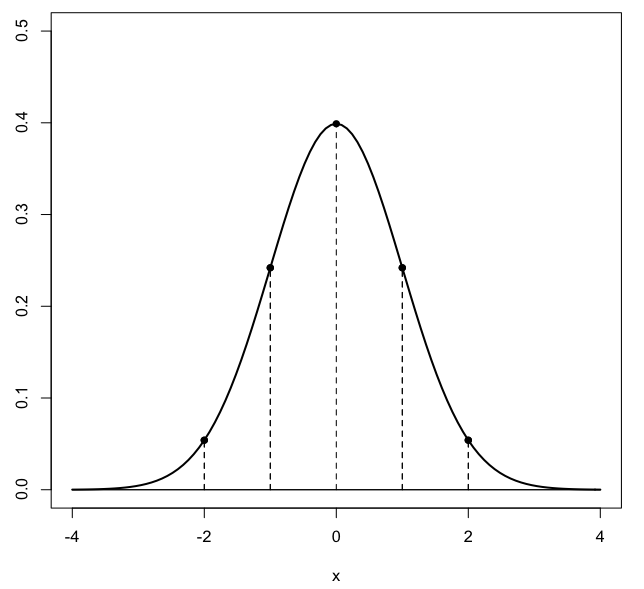
\includegraphics [scale=0.4] {gauss3.png} \end{center}
% \begin{bmatrix} a  &  b \\ c  &  d \end{bmatrix}
% \bigg |_

\begin{document}
\maketitle
\large
%\noindent

I'm trying to reproduce here the argument I saw in a video by Math Dr. Bob about this subject.  

We know already know how to calculate values for sine and cosine of $\pi$ times $\frac{1}{2}$, $\frac{1}{3}$, $\frac{1}{4}$, and $\frac{1}{6}$, and various increments multiplied by $n=2,3 \cdots$.  The next obvious target is $\frac{1}{5} \pi$.  

It turns out this can also be done pretty easily, and it leads to an interesting connection, which can be reached from a different perspective by looking at the properties of pentagons (remember that the interior angle of a pentagon is $\pi - \frac{2}{5} \pi = \frac{3}{5} \pi$.

Begin by writing down the double angle formulas for sine and cosine:
\[ \sin 2s = 2 \sin s \cos s \]
\[ \cos 2s = \cos^2s - \sin^2s = 2 \cos^2 s - 1 \]

If you visualize (or sketch) going around the unit circle in increments of $2 \pi /5$, you will see that $\theta = \frac{2}{5} \pi$ and $\phi = 4 \theta = \frac{8}{5} \pi$ form the same angle with the $x$-axis (convention adds a factor of -1).  Therefore, these two angles have the same cosine, and   the same sine as well, except for that factor of -1.  For this particular angle $\theta =\frac{2}{5} \pi$

\[ -\sin \theta = \sin 4 \theta \]

Next, we use the double angle formulas to write out an expression for $\sin 4 \theta$

\[ \sin 4 \theta = 2 \ (\sin 2 \theta)(\cos 2 \theta) \]
\[  = 2 \ (2 \sin \theta \cos \theta)(2 \cos^2 \theta - 1) \]

Combining with what we had before

\[   -\sin \theta = 2 (2 \sin \theta \cos \theta)(2 \cos^2 \theta - 1) \]

Factor out $\sin \theta$

\[   -1 = 2 (2 \cos \theta)(2 \cos^2 \theta - 1) \]

Substituting $x = \cos \theta$

\[   -1 = 2 (2 x)(2 x^2 - 1) \]
\[   -1 = 8 x^3 - 4x  \]
\[    8 x^3 - 4x + 1 = 0 \]

Now, it turns out that $x = \frac{1}{2}$ is a solution of this polynomial (easily checked), so we should be able to factor it into something like

\[    8 x^3 - 4x + 1 = (x - \frac{1}{2}) (\cdots)  \]

We deduce the rest of the factorization:

\[    8 x^3 - 4x + 1 = (x - \frac{1}{2}) (8x^2 \cdots)  \]
\[    8 x^3 - 4x + 1 = (x - \frac{1}{2}) (8x^2+ 4x \cdots )  \]
\[    8 x^3 - 4x + 1 = (x - \frac{1}{2}) (8x^2+ 4x -2 )  \]

We can get the solutions for the second factor

\[ 8x^2+ 4x -2 \]

from the quadratic equation:

\[ \frac{-4 \pm \sqrt{16 + 4(16)}}{16} \]
\[ - \frac{1}{4} (1 \pm \frac{1}{4} \sqrt{16 + 4(16)} ) \]
\[ - \frac{1}{4} (1 \pm \sqrt{\frac{16 + 4(16)}{16}} ) \]
\[ - \frac{1}{4} (1 \pm \sqrt{5} ) \]
\[ - \frac{1}{2}  \ ( \frac{1 \pm \sqrt{5}}{2} ) \]
\[ - \frac{1}{2} \phi_1,  - \frac{1}{2} \phi_2 \]

where
\[ \phi_1 =   \frac{1 + \sqrt{5} }{2} \approx  1.618034 \]
\[ \phi_2 =   \frac{1 - \sqrt{5} }{2} \approx  -0.618034 \]

What does this mean?  It means that if
\[ -\sin \theta = \sin 4 \theta \]
then solutions include $\theta$ for which

\begin{equation*}
    \cos \theta = \begin{cases}
              \ \  \frac{1}{2}  \\
               -\frac{1}{2} \phi_1 \\
               -\frac{1}{2} \phi_2 \\
           \end{cases}
\end{equation*}

The third solution is numerically:
\[ -\frac{1}{2} \ (-0.618034) = 0.309017 \]
                 
And the cosine of $2 \pi /5$ is equal to 0.309017, which checks!

Another way to obtain this result is to start from our work with the pentagon.  

\begin{center} 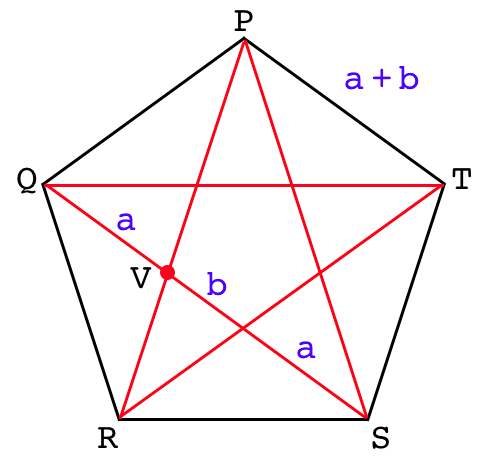
\includegraphics [scale=0.4] {pentagon.png} \end{center}

We draw the chords of the pentagon, then consider the smallest triangle obtained.  It is isosceles with two sides $a$ and the last side $b$.  The two larger angles measure $2 \pi/5$ and the other is $\pi/5$.  The law of cosines gives:

\[ a^2 = a^2 + b^2 - 2 a b \cos \ (\frac{2}{5}\pi)\]
\[ -b^2 = -2 ab \ \cos \ (\frac{2}{5}\pi) \]
\[ \frac{b}{a} =  2 \cos \ (\frac{2}{5}\pi)\]

and in the writeup about pentagons, what we found was that

\[ \frac{a}{b} = \phi_1 \]

so
\[ \cos \ (\frac{2}{5}\pi) = -\frac{1}{2} \ \frac{1}{\phi_1 } =  -\frac{1}{2} \ \phi_2 \]

The last step follows since $\phi_1 \ \phi_2 = -1$.

\end{document}  